\begin{figure*}

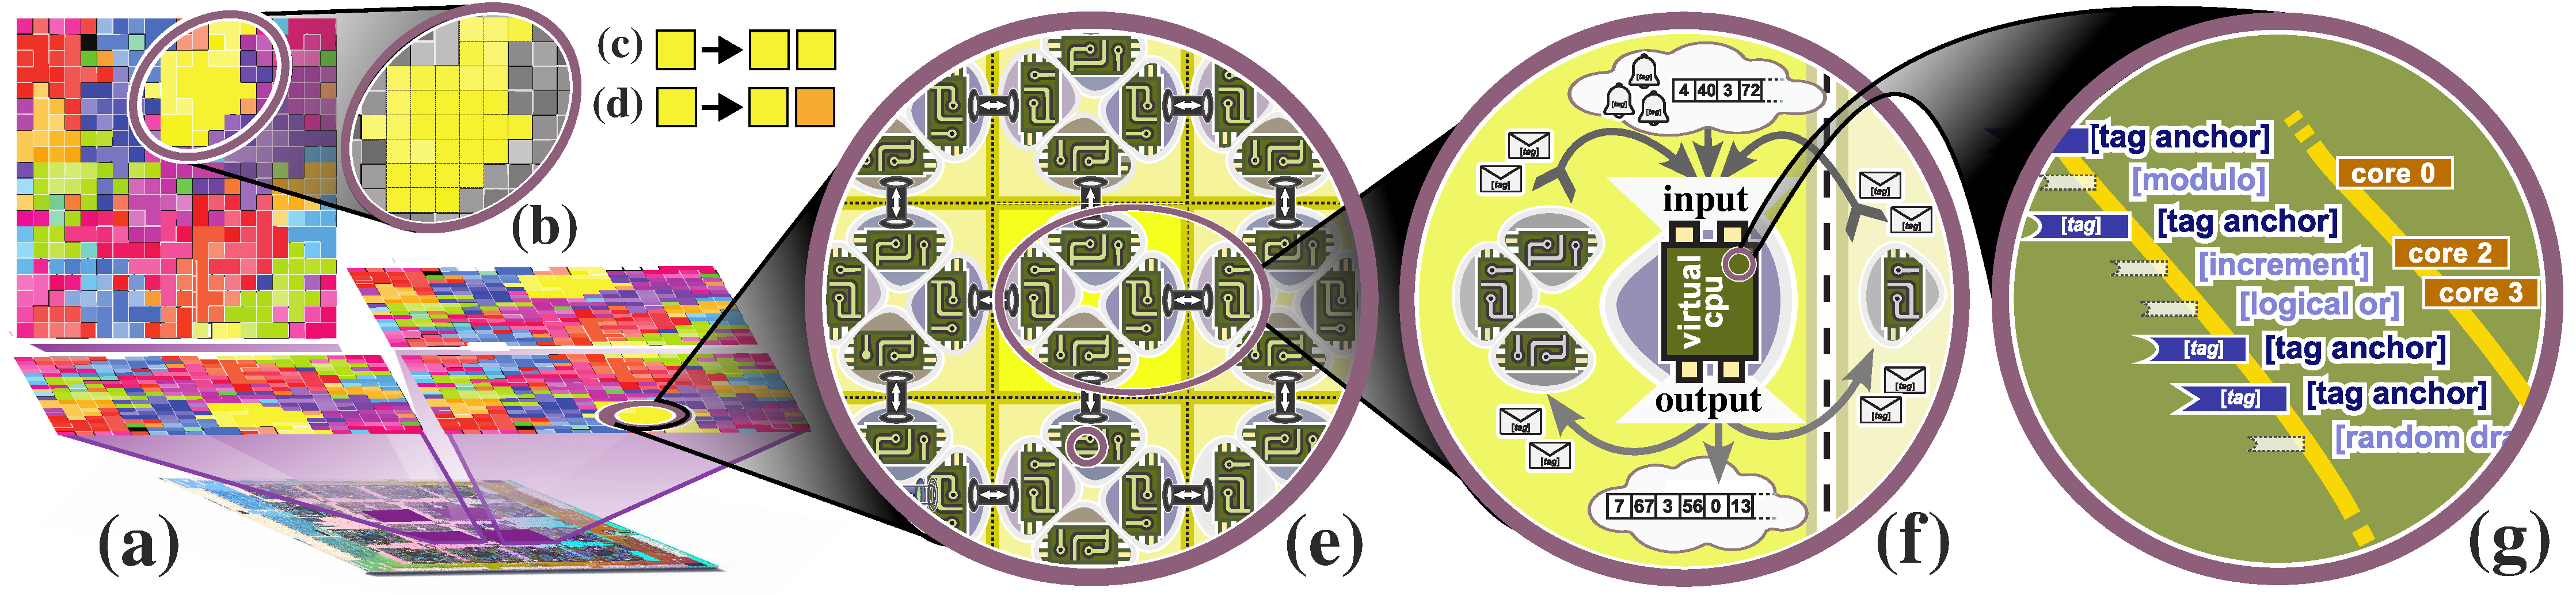
\includegraphics[width=\linewidth]{{img/graphic-oee4-cpu.pdf}}

\caption{
\textbf{Overview of digital multicell model.}
\footnotesize
Population comprises a toroidal grid of cells occupied by replicating computer programs.
In the surveyed case study, grid size was 14,400 cells ($120\times120$).
To accelerate the feasible evolutionary depth of experiments, population subgrids are evaluated across available hardware threads and processes --- in this work, 4 threads (panel $a$).
At subgrid boundaries where inter-cell interactions reach between different threads or processes, communication is handled on a best-effort basis via the underlying Conduit library.
On the population grid, cells may form local multicell groups --- shown as colored patches in visualizations (panel $b$).
Cells replicate by copying program content into a chosen neighbor cell, and may choose to grow their existing multicell group ($c$) --- or splinter their offspring off to found a new group ($d$).
Within each cell, behavior is directed by a collection of four virtual CPUs (N, S, E, and W ``cardinal processors''), each independently managing the cell's interactions with a one neighbor cell (panel $c$).
Each cardinal processor can interact with other cardinal processors in its own cell via message passing.
A cardinal processor can also exchange messages with its counterpart cardinal processor in the abutting neighbor cell, allowing arbitrary inter-cell communication.
Alongside message-passing I/O, cardinal processors accept input to sense local simulation state and create output to perform cell actions (panel $f$).
Sensory input occurs via a combination of special input registers (e.g., for own- and neighbor-cell resource availability, cell age, etc.) and special messages triggered by simulation conditions (``events,'' depicted as bells in panel $f$).
Behavior outputs are dispatched via special output registers (e.g., for resource sharing, replication, apoptosis, etc.).
At implementation level, replicator program code is evaluated via an event-driven execution model.
That is, tag-matching mechanisms trigger program submodules in response to stimuli (panel $g$).
In addition to external stimuli (i.e., inter-cellular messages, intra-cellular messages, and simulation events), program code can also trigger arbitrary self-stimuli.
Virtual hardware supports concurrent interaction handling via independent pseudo-cores, as well as dynamic plasticity through regulation of tag-matching affinities within each cardinal processor.
}
\label{fig:overview}
\end{figure*}
